../cictikz/src/cictikz/data/tex/cictikz_preamble.tex

% Gate voltage against gm/ID, over the useful range.
%
% This is the plot to design from: pick a gm/ID and read off the bias
% voltage the device needs.
%
% Generated by py/tikzplot.py. Edit the script in ex/ that
% produced it and re-run that, not this file.

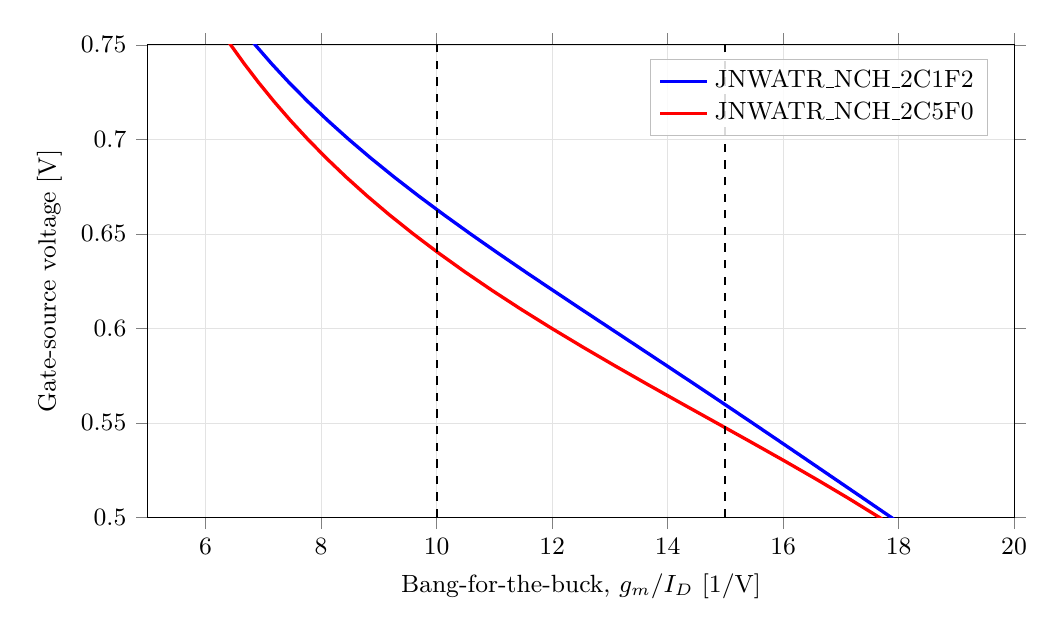
\begin{tikzpicture}[thick]

\begin{axis}[
  width=11.0cm,
  height=6.0cm,
  scale only axis,
  grid=both,
  grid style={gray!22, very thin},
  tick align=outside,
  tick label style={font=\small},
  label style={font=\small},
  title style={font=\small, yshift=-1mm},
  legend cell align=left,
  legend style={font=\small, draw=gray!50, fill=white, fill opacity=0.85, text opacity=1},
  xlabel={Bang-for-the-buck, $g_m/I_D$ [1/V]},
  ylabel={Gate-source voltage [V]},
  xmin=5,
  xmax=20,
  ymin=0.5,
  ymax=0.75,
  legend pos=north east
]
\addplot[blue, very thick, mark=none] coordinates {(27.373,0) (27.341,0.01) (27.309,0.02) (27.277,0.03) (27.244,0.04) (27.21,0.05) (27.176,0.06) (27.14,0.07) (27.104,0.08) (27.066,0.09) (27.027,0.1) (26.987,0.11) (26.944,0.12) (26.9,0.13) (26.853,0.14) (26.804,0.15) (26.751,0.16) (26.695,0.17) (26.635,0.18) (26.571,0.19) (26.501,0.2) (26.425,0.21) (26.343,0.22) (26.252,0.23) (26.154,0.24) (26.045,0.25) (25.925,0.26) (25.794,0.27) (25.649,0.28) (25.489,0.29) (25.313,0.3) (25.119,0.31) (24.906,0.32) (24.674,0.33) (24.42,0.34) (24.144,0.35) (23.845,0.36) (23.524,0.37) (23.18,0.38) (22.814,0.39) (22.427,0.4) (22.021,0.41) (21.597,0.42) (21.159,0.43) (20.707,0.44) (20.246,0.45) (19.778,0.46) (19.305,0.47) (18.828,0.48) (18.35,0.49) (17.872,0.5) (17.393,0.51) (16.913,0.52) (16.433,0.53) (15.951,0.54) (15.467,0.55) (14.98,0.56) (14.49,0.57) (13.997,0.58) (13.502,0.59) (13.007,0.6) (12.512,0.61) (12.02,0.62) (11.533,0.63) (11.054,0.64) (10.586,0.65) (10.131,0.66) (9.6907,0.67) (9.2679,0.68) (8.8637,0.69) (8.4791,0.7) (8.1148,0.71) (7.771,0.72) (7.4474,0.73) (7.1435,0.74) (6.8585,0.75) (6.5915,0.76) (6.3414,0.77) (6.1069,0.78) (5.8871,0.79) (5.6808,0.8) (5.4869,0.81) (5.3044,0.82) (5.1324,0.83) (4.9701,0.84) (4.8168,0.85) (4.6717,0.86) (4.5343,0.87) (4.404,0.88) (4.2802,0.89) (4.1626,0.9) (4.0507,0.91) (3.944,0.92) (3.8424,0.93) (3.7454,0.94) (3.6527,0.95) (3.564,0.96) (3.4792,0.97) (3.3979,0.98) (3.32,0.99) (3.2452,1) (3.1734,1.01) (3.1044,1.02) (3.0381,1.03) (2.9742,1.04) (2.9127,1.05) (2.8534,1.06) (2.7963,1.07) (2.7411,1.08) (2.6879,1.09) (2.6364,1.1) (2.5866,1.11) (2.5385,1.12) (2.492,1.13) (2.4469,1.14) (2.4032,1.15) (2.3609,1.16) (2.3198,1.17) (2.28,1.18) (2.2414,1.19) (2.2039,1.2) (2.1674,1.21) (2.132,1.22) (2.0976,1.23) (2.0641,1.24) (2.0316,1.25) (1.9999,1.26) (1.9691,1.27) (1.9391,1.28) (1.9098,1.29) (1.8813,1.3) (1.8536,1.31) (1.8265,1.32) (1.8001,1.33) (1.7744,1.34) (1.7492,1.35) (1.7247,1.36) (1.7008,1.37) (1.6774,1.38) (1.6546,1.39) (1.6323,1.4) (1.6105,1.41) (1.5892,1.42) (1.5684,1.43) (1.5481,1.44) (1.5282,1.45) (1.5087,1.46) (1.4896,1.47) (1.471,1.48) (1.4528,1.49) (1.4349,1.5) (1.4174,1.51) (1.4003,1.52) (1.3835,1.53) (1.3671,1.54) (1.351,1.55) (1.3352,1.56) (1.3197,1.57) (1.3046,1.58) (1.2897,1.59) (1.2751,1.6) (1.2608,1.61) (1.2468,1.62) (1.2331,1.63) (1.2196,1.64) (1.2063,1.65) (1.1933,1.66) (1.1805,1.67) (1.168,1.68) (1.1557,1.69) (1.1436,1.7) (1.1318,1.71) (1.1201,1.72) (1.1086,1.73) (1.0974,1.74) (1.0863,1.75) (1.0755,1.76) (1.0648,1.77) (1.0543,1.78) (1.044,1.79) (1.0338,1.8)};
\addlegendentry{JNWATR\_NCH\_2C1F2}
\addplot[red, very thick, mark=none] coordinates {(28.345,0) (28.302,0.01) (28.258,0.02) (28.214,0.03) (28.168,0.04) (28.121,0.05) (28.072,0.06) (28.022,0.07) (27.97,0.08) (27.916,0.09) (27.86,0.1) (27.802,0.11) (27.74,0.12) (27.675,0.13) (27.606,0.14) (27.532,0.15) (27.453,0.16) (27.369,0.17) (27.277,0.18) (27.178,0.19) (27.07,0.2) (26.953,0.21) (26.824,0.22) (26.683,0.23) (26.529,0.24) (26.359,0.25) (26.174,0.26) (25.971,0.27) (25.75,0.28) (25.509,0.29) (25.249,0.3) (24.97,0.31) (24.671,0.32) (24.355,0.33) (24.022,0.34) (23.676,0.35) (23.319,0.36) (22.953,0.37) (22.583,0.38) (22.211,0.39) (21.838,0.4) (21.466,0.41) (21.093,0.42) (20.717,0.43) (20.334,0.44) (19.941,0.45) (19.532,0.46) (19.103,0.47) (18.65,0.48) (18.171,0.49) (17.666,0.5) (17.136,0.51) (16.585,0.52) (16.016,0.53) (15.435,0.54) (14.847,0.55) (14.258,0.56) (13.674,0.57) (13.099,0.58) (12.538,0.59) (11.993,0.6) (11.468,0.61) (10.965,0.62) (10.485,0.63) (10.028,0.64) (9.5947,0.65) (9.1852,0.66) (8.7989,0.67) (8.4351,0.68) (8.0929,0.69) (7.7713,0.7) (7.4692,0.71) (7.1856,0.72) (6.9192,0.73) (6.6691,0.74) (6.4342,0.75) (6.2133,0.76) (6.0056,0.77) (5.8101,0.78) (5.6259,0.79) (5.4522,0.8) (5.2883,0.81) (5.1334,0.82) (4.9868,0.83) (4.848,0.84) (4.7165,0.85) (4.5916,0.86) (4.4729,0.87) (4.36,0.88) (4.2524,0.89) (4.1498,0.9) (4.0519,0.91) (3.9583,0.92) (3.8687,0.93) (3.7829,0.94) (3.7007,0.95) (3.6217,0.96) (3.5459,0.97) (3.4729,0.98) (3.4028,0.99) (3.3351,1) (3.27,1.01) (3.207,1.02) (3.1463,1.03) (3.0876,1.04) (3.0309,1.05) (2.9759,1.06) (2.9227,1.07) (2.8712,1.08) (2.8213,1.09) (2.7728,1.1) (2.7258,1.11) (2.6801,1.12) (2.6357,1.13) (2.5926,1.14) (2.5506,1.15) (2.5098,1.16) (2.4701,1.17) (2.4314,1.18) (2.3937,1.19) (2.357,1.2) (2.3212,1.21) (2.2863,1.22) (2.2523,1.23) (2.219,1.24) (2.1866,1.25) (2.1549,1.26) (2.1239,1.27) (2.0937,1.28) (2.0642,1.29) (2.0353,1.3) (2.007,1.31) (1.9794,1.32) (1.9524,1.33) (1.9259,1.34) (1.9,1.35) (1.8747,1.36) (1.8499,1.37) (1.8256,1.38) (1.8018,1.39) (1.7784,1.4) (1.7556,1.41) (1.7332,1.42) (1.7112,1.43) (1.6897,1.44) (1.6686,1.45) (1.6478,1.46) (1.6275,1.47) (1.6076,1.48) (1.588,1.49) (1.5688,1.5) (1.55,1.51) (1.5315,1.52) (1.5133,1.53) (1.4955,1.54) (1.478,1.55) (1.4607,1.56) (1.4438,1.57) (1.4272,1.58) (1.4109,1.59) (1.3949,1.6) (1.3791,1.61) (1.3636,1.62) (1.3483,1.63) (1.3334,1.64) (1.3186,1.65) (1.3041,1.66) (1.2899,1.67) (1.2759,1.68) (1.2621,1.69) (1.2485,1.7) (1.2352,1.71) (1.222,1.72) (1.2091,1.73) (1.1964,1.74) (1.1838,1.75) (1.1715,1.76) (1.1594,1.77) (1.1474,1.78) (1.1356,1.79) (1.1241,1.8)};
\addlegendentry{JNWATR\_NCH\_2C5F0}
\draw[black, dashed, thick] ({axis cs:10,0} |- {rel axis cs:0,0}) -- ({axis cs:10,0} |- {rel axis cs:0,1});
\draw[black, dashed, thick] ({axis cs:15,0} |- {rel axis cs:0,0}) -- ({axis cs:15,0} |- {rel axis cs:0,1});
\end{axis}

\end{tikzpicture}
\end{document}
